\chapter{基于物理渲染和着色的理论基础}

光是一种非常复杂的自然现象,能够同时展现出波动性质和粒子性质,迄今为止已经有很多不同的模型被提出来解释光的行为。对于纹理艺术家来说,我们关注的是最简单的光线模型(也就是大家都明白的:光沿直线传播)所描述的光与物体表面的互动。纹理艺术家的工作就是创造描述物体表面性质的纹理贴图,所以自然知道光和物体互动的理论是非常重要的。
这篇导读中,我们会讨论作为基于物理渲染(PBR)的理论基础的一些物理“常识”。首先我们自然是从光线模型,这一PBR的核心因素入手。

\section{光线是啥}

光线模型基于一个众所周知的真理:光线在相同的介质中的轨迹是绝对的直线,比如在空气中就是如此。光线模型还告诉我们光在物体表面的行为是可以预测的,包括在不透明物体表面的反射、在穿过不同介质界面的折射等。这就让我们能够完整的在虚拟世界中模拟一条光线的生命周期,从它的起点一直到它最后因为散射而衰竭变成热量,我们在计算机中都可以编写相应的模型去计算。

击中物体表面的光线叫做入射光线,如图\ref{fig:chap1_1}所示的,而光线和物体表面法线所成的角叫做入射角。

\begin{figure}[ht]
    \centering
	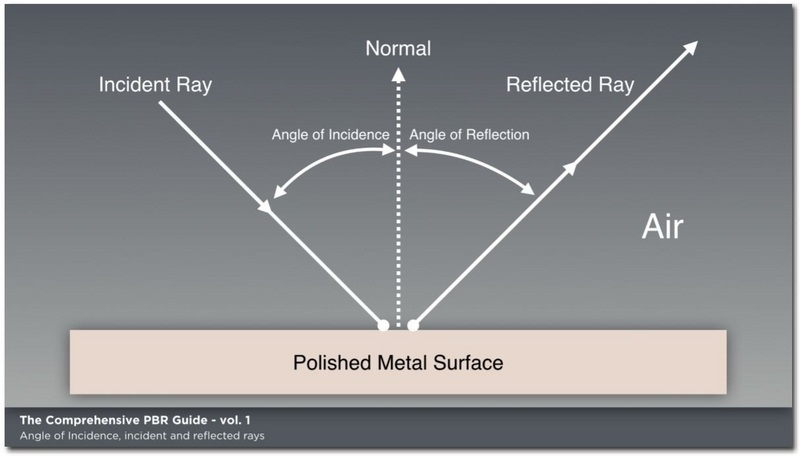
\includegraphics[width=\textwidth]{images/chap1_1.jpg}
	\caption{入射、反射光线及入射角度}
    \label{fig:chap1_1}
\end{figure}

当光线击中表面时,一般有两件事情可能会发生:

\begin{enumerate}
\item 光线根据反射定律被表面完全反射并被弹向一个完全不同的角度,反射角度等于入射角度。
\item 光线按折线形式由一种介质传播到另一种介质。这时光线被分成折射和反射的两部分。在物体表面,光线同时存在被反射和折射的可能性,其中折射的光线可能最终被介质吸收,当然,吸收衰竭的过程不会发生在物体表面。
\end{enumerate}

\section{吸收与散射(透明和半透明)}

当光线在各向异性的介质(也就是半透明物体)中传播时,光线可能会被吸收或者散射:

\begin{enumerate}
\item 当光线在介质中被吸收时,光能量随着它被转换成其他形式的能量而衰竭(通常是热量),光的颜色(波长)也会根据介质的吸收特性而改变,但光线传播的方向不变。
\item 当光线在介质中被散射时,光线传播方向会随机变化,其方向的变化幅度取决于介质的性质。散射会让光的传播方向随机发生变化但是光线强度却不变。一个生物体组织的耳朵是一个很好的散射例子。耳朵很薄(吸收效应很弱),所以我们能够从耳朵背面看见散射的光线穿透过来(血红色)。假如没有散射并且吸收效应很弱的话,耳朵会看起来像像玻璃一样透明。另一个例子是游泳池,如果泳池的水足够清澈,那么你在其中游泳时可以在水下看的很远,这时我们可以认为水是透明的。反之,如果是一池脏水,水中的污物粒子就会大大加剧散射的效应,这时候水的透明度就会变得非常低。
\end{enumerate}

光线在介质中传播的越远,散射和吸收带来的损失就会越多,因此,\textbf{物体的厚度在光线的散射和吸收中扮演了重要角色},图\ref{fig:chap1_2}用了一张厚度贴图来在shader中表示物体厚度(用于计算散射强度)。

\begin{figure}[ht]
    \centering
	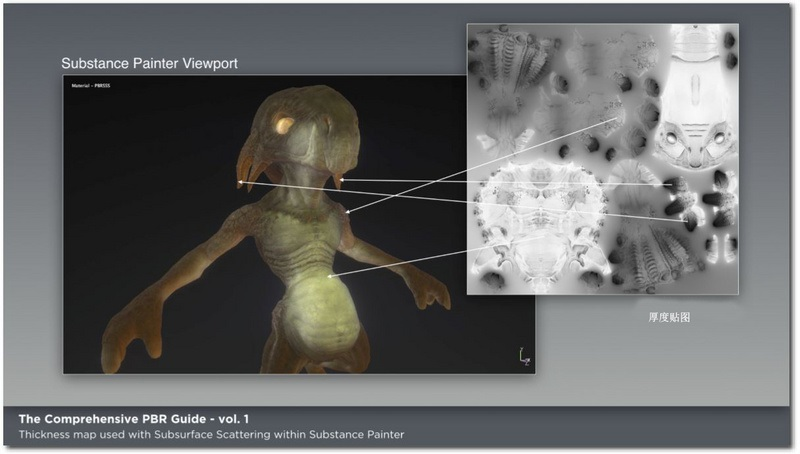
\includegraphics[width=\textwidth]{images/chap1_2.jpg}
	\caption{Substance Painter中用于次表面反射的厚度图}
    \label{fig:chap1_2}
\end{figure}

\section{漫反射与高光反射}

高光反射用来描述的是我们之前提到的光被物体表面反弹出去的想象,光线被物体表面反射到一个完全不同的角度之后的现象。无论是漫反射还是高光反射都遵从着描述完美镜面反射现象的反射定律。然而,由于物体表面往往并不能像完美镜面一样光滑,光线反射出去的方向往往是非常随机的。而反射光线的随机程度与物体表面的粗糙程度成正相关。漫反射与高光反射改变了光源发出的光的方向,但并不改变其强度。

粗糙表面的反射呈现出更大范围而且相对较暗的高光区域,而光滑表面的高光反射则更加集中和明亮。当然,两种表面反射的光的总量是一致的,如图\ref{fig:chap1_3}所示。

\begin{figure}[ht]
    \centering
	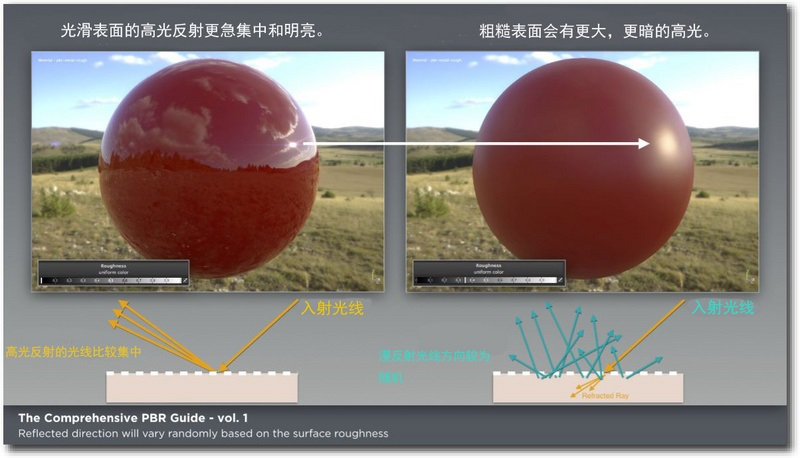
\includegraphics[width=\textwidth]{images/chap1_3.jpg}
	\caption{根据表面粗糙度,光线会随机反射}
    \label{fig:chap1_3}
\end{figure}

在完全的漫反射现象中,光线其实已经被折射至物体内部,并在新的介质中经历多次散射,之后再次从物体内部折射而出,而折射出点和光线入射点往往距离非常接近,如图\ref{fig:chap1_4}所示。

\begin{figure}[ht]
    \centering
	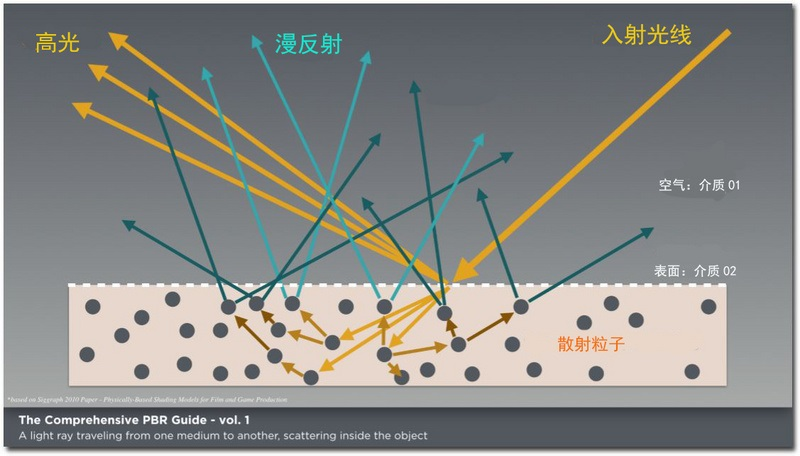
\includegraphics[width=\textwidth]{images/chap1_4.jpg}
	\caption{光线从一个介质到另一个时,在内部发生了散射}
    \label{fig:chap1_4}
\end{figure}

漫反射性质的物体往往对光线更加具有吸收性质,光线甚至很有可能被其完全吸收(在材质中走的够远的话)。这也就意味着漫反射出去的光线并没有在物体材质中传播多远,因此入射点和出射点之间的距离才可以忽略。传统渲染着色模型中常用的Lambertian模型,并没有将表面粗糙度考虑在其中,但新的漫反射模型比如Oren-Nayar就将物体粗糙度也作为一个参数。

相对应的,拥有很高散射系数和相对较低的吸收率的物体材质就被称为“参于介质”或者更通俗的“半透明物体”。例如烟,牛奶,皮肤,玉石和大理石。渲染后三种物体可以采用次表面散射的模型处理,当渲染这三种材质时入射点和出射点的距离就不再能够被忽略。正确渲染高度各向异性和低散射吸收系数的物体比如烟和雾往往需要更加昂贵的方法,比如蒙特卡洛模拟。

\section{微平面理论}

理论上来说,无论是漫反射或者高光反射都与反射光线表面的粗糙和崎岖程度有关系,对于漫反射表面来说,粗糙程度对反射的影响要小的很多因为光线往往在物体内部发生散射,结果就是漫反射表面的出射光线往往展现出一种与入射角和粗糙程度无关的随机性。最常用的Lambertian模型就是基于这样的现象建立的理论。

这篇文档中,我们把物体表面和光滑平面的差异和不规则程度:如凹凸不平。叫做粗糙度。实际上,它根据PBR工作流的不同又被称为粗糙度,光泽度,高光度等等。但它们都描述了物体表面次像素级别的同一种属性。

在实际的PBR工作流中,这种物体表面的不规则性被一张粗糙度贴图或者高光度贴图来表示。微平面理论,一种把物体表面看做无数微观尺度,但有着随机朝向的理想反射镜面来建模的理论,推导出了一个基于粗糙度的BRDF公式(见后文)来描述物体的反射。在这个理论中,每个微平面都像完美镜面一样基于自己的法线把光线反射向同一个方向,如图\ref{fig:chap1_5}。

\begin{figure}[ht]
    \centering
	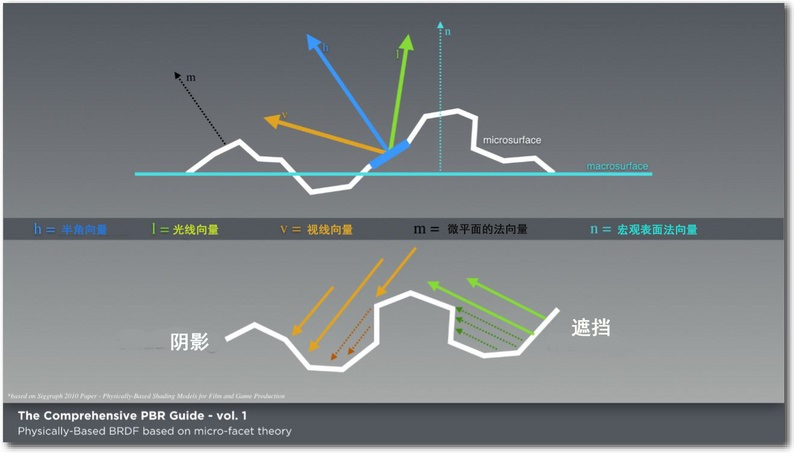
\includegraphics[width=\textwidth]{images/chap1_5.jpg}
	\caption{基于微面理论的基于物理的BRDF}
    \label{fig:chap1_5}
\end{figure}

对于每一个微小平面来说,其表面法线严格朝向光线方向和视线方向的中间,然而并不是所有的微小平面的法线与半角向量相同。如图\ref{fig:chap1_5}所示,微小平面之间存在着阴影(对于光照方向来说)和遮挡(对于视线方向来说)。

\textbf{物体表面在微观层级的不规则性造成了光线的扩散}。比如,模糊的反射就是因为被散射的光线,被反射的光线如果不是平行的,看上去就会和被模糊一样。如图\ref{fig:chap1_6}所示。

\begin{figure}[ht]
    \centering
	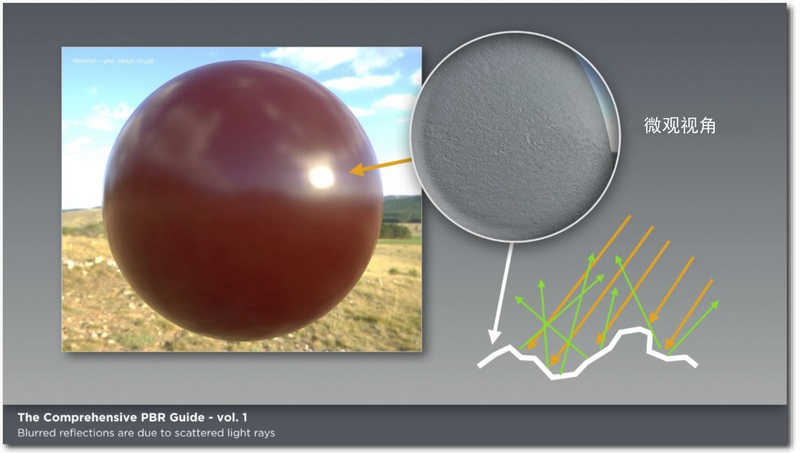
\includegraphics[width=\textwidth]{images/chap1_6.jpg}
	\caption{光线散射将导致反射模糊}
    \label{fig:chap1_6}
\end{figure}

\section{颜色}

物体表面的颜色(也就是我们的肉眼所看到的颜色),来自于光线的波长。光源发出的光线在经过物体的吸收后反射出来的光线(包括高光和漫反射)最后进入眼睛的光线的波长就是我们看到的颜色。

例如:红苹果的皮最多反射的是红色光线,只有红光在散射后被弹出,而其他波长的光线都被苹果吸收了,如图\ref{fig:chap1_7}。

\begin{figure}[ht]
    \centering
	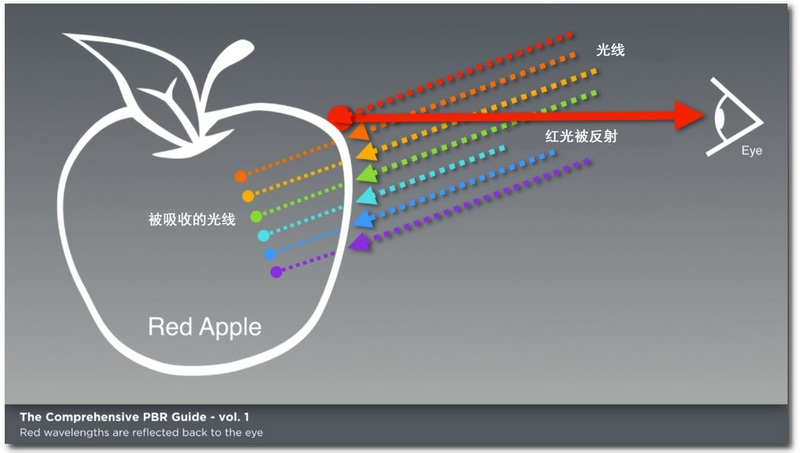
\includegraphics[width=\textwidth]{images/chap1_7.jpg}
	\caption{红色波长被反射回人眼}
    \label{fig:chap1_7}
\end{figure}

苹果表面同时还有和光源颜色一样的高光。这是因为苹果皮并非导体,高光反射几乎与光线波长无关。因此这样物体的高光反射一般来说不会带有物体自身的颜色,后续章节会讨论不同种类物质之间反射的区别。

\section{BRDF}

双向反射分布函数(BRDF)是一个描述物体表面反射性质的函数。计算机图形学中有很多BRDF模型是与实际物理无关。对于一个基于物理的BRDF模型(注:物理合理或者说基于物理的模型,并不是物理精确的,而是满足若干项物理性质,能更好进行建模工作的模型),它必须是能量守恒并且是显式可逆的,可逆性质,也就是光路的可逆性,是指入射光和出射光可以被认为是互相可以代替并且不影响BRDF的值的性质。

Substance shader采用的是迪斯尼提出的基于GGX微平面分布的反射模型。GGX微平面分布对高光反射做了一个非常棒的近似,它在高光峰值处有一个很小的尖峰,并且在衰竭时有“长尾”,看起来会非常真实,如图\ref{fig:chap1_8}。

\begin{figure}[ht]
    \centering
	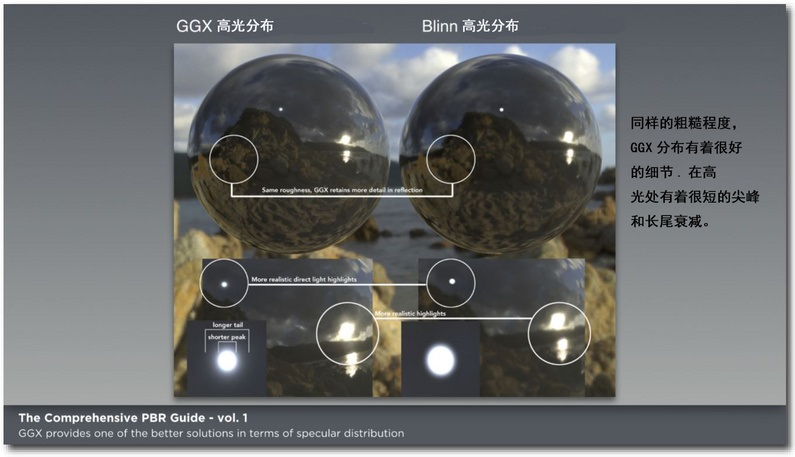
\includegraphics[width=\textwidth]{images/chap1_8.jpg}
	\caption{GGX在高光项提供了更好的近似}
    \label{fig:chap1_8}
\end{figure}

\section{能量守恒}

能量守恒在基于物理的渲染解决方案中扮演着至关重要的作用。它所表达的规律是从物体表面反射或者散射的光的总量总是小于表面接收到的光的总量,或者说被反射出去的光线强度永远不会有入射光线那么高。对于艺术家来说,我们并不需要考虑去控制能量守恒的问题。这是因为能量守恒总是在PBR shader里被考虑了。能量守恒是基于物理模型的一部分,让我们更多的集中注意力在艺术创造而不是物理。

\section{菲涅尔效应}

菲涅尔效应在基于物理渲染模型的BRDF中扮演着一个重要的因子。菲涅尔效应得名于观测到这种现象的法国物理学家让.奥古斯丁.菲涅尔。它表示的是你看到的反射光线的量与你和视角相关的现象。

一个很好的例子是一池清水,从水池上笔直看下去(也就是与法线成零度角的方向)的话,我们能够一直看到池底。而如果从接近平行于水面的方向看去的话,水池表面的高光反射会变得非常强以至于你看不到池底。菲涅尔效应和能量守恒一样是由PBR shader处理的。当从接近平行于表面的视线方向看过去时,所有光滑表面都会变得100\%的反射性。

对于粗糙表面来说,在接近平行方向的高光反射也会增强但不够达到100\%的强度.为何如此是因为影响菲涅尔效应的关键参数在于每个微平面的法向量和入射光线的角度,而不是宏观平面的法向量和入射光线的角度。因此我们在宏观层面看到的实际上是微平面的菲涅尔效应的一个平均结果。

\section{F0(0度角菲涅尔反射值)}

当光线垂直打中物体表面(与法向量成零度角)时,有一部分光被直接反弹回去成为高光。根据表面折射率(IOR值)我们可以推导出这个角度被反射的光的量,我们称之为F0,如图\ref{fig:chap1_9}.而剩余被折射进物体的光就被称作1-F0。

\begin{figure}[ht]
    \centering
	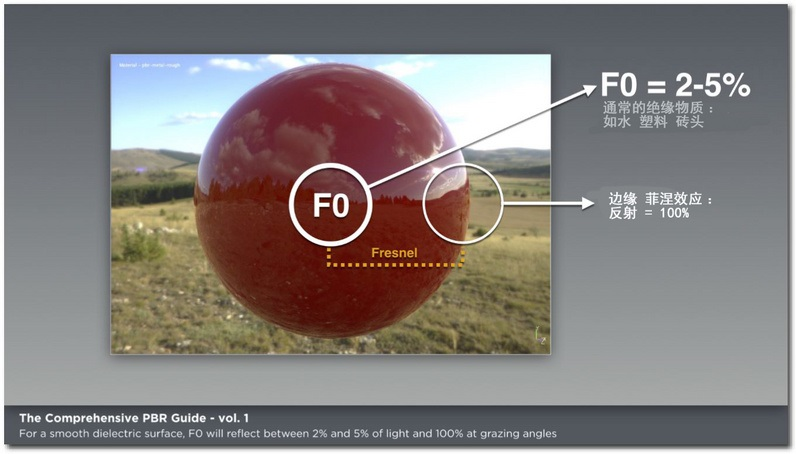
\includegraphics[width=\textwidth]{images/chap1_9.jpg}
	\caption{对于一个光滑的绝缘表面,F0会切线角反射100\%、在垂直面反射2\%-5\%的入射光}
    \label{fig:chap1_9}
\end{figure}

大多数绝缘体的F0范围在0.02-0.05,导体的F0范围则可高达0.5-1.0.推导F0的公式如图\ref{fig:chap1_10}所示。

\begin{figure}[ht]
    \centering
	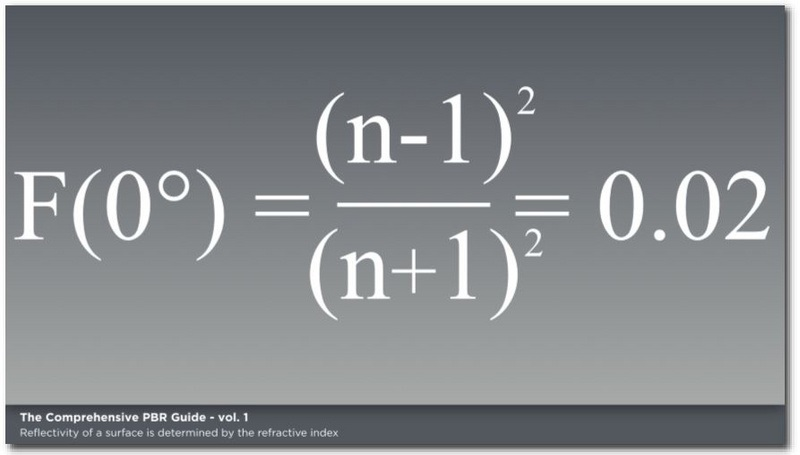
\includegraphics[width=\textwidth]{images/chap1_10.jpg}
	\caption{平面的反射率由其折射率决定}
    \label{fig:chap1_10}
\end{figure}

F0在我们创造纹理的过程中起着很重要的作用,非金属的F0值会是一个灰度值(对所有波长的光同等反射)金属的F0值则会是一个RGB值。实际应用中我们可以说大部分光滑绝缘物体表面的F0在2\%-5\%而在平视角度反射达到100\%(图\ref{fig:chap1_9})。

绝缘体的菲涅尔反射值实际上往往变化不大,以至于往往很难观察到。图\ref{fig:chap1_11}展示了从非金属到金属的F0值的范围变化。

\begin{figure}[ht]
    \centering
	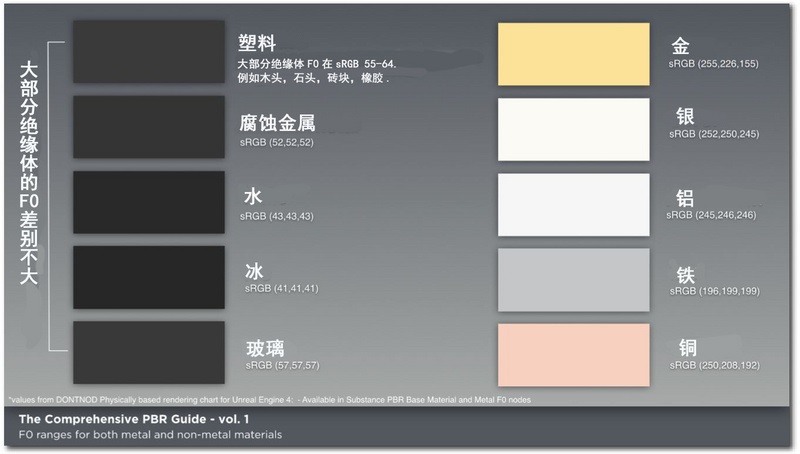
\includegraphics[width=\textwidth]{images/chap1_11.jpg}
	\caption{金属、非金属材质的F0变化}
    \label{fig:chap1_11}
\end{figure}

注意除了宝石之外的大部分绝缘体的F0值相差并不大,后续我们会讨论导体和绝缘体之间的F0差异。

\section{导体和绝缘体}

当在创造PBR材质的时候,用金属和非金属的方式去思考分类物体是非常有用的。只要简单的区分物体表面是金属还是非金属,如果是,那么按照一套规则去制作纹理,反之亦然。这种方面可能会存在例外因为有些物质不能进行简单的区分,但是在大部分创作材质的情况下,按照金属和非金属进行区别是一种有效的手段。根据PBR理论,我们可以推导出金属和非金属的属性,并进一步推导出创造这两类物质的纹理的准则。

\section{金属}

金属是热和电的良导体。一个物理知识:金属内部的电场强度总是0,因此当外来的电磁波击中金属时(比如光线),大部分光线会被反弹而剩余的则被完全吸收。因此,对于抛光金属反射率往往能达到70\%到100\%。如图\ref{fig:chap1_12}.

\begin{figure}[ht]
    \centering
	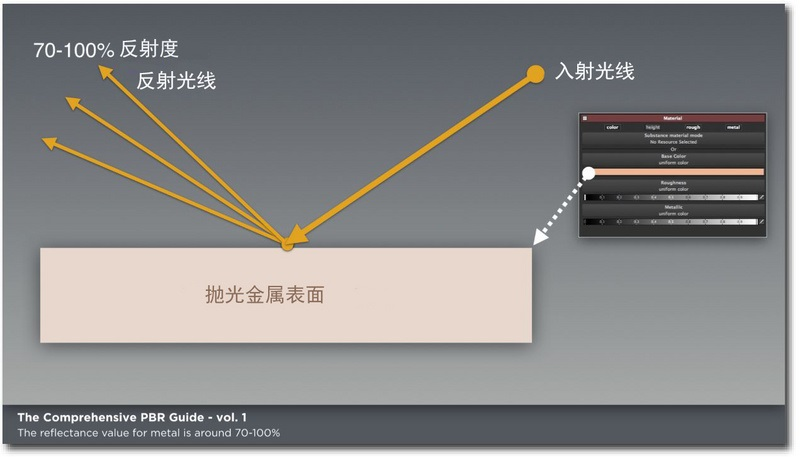
\includegraphics[width=\textwidth]{images/chap1_12.jpg}
	\caption{金属反射度大概在70\%-100\%}
    \label{fig:chap1_12}
\end{figure}

有些金属对光线波长有着选择性吸收,例如金会吸收高波长的光线比如蓝光因此金看上去呈现黄色。由于折射的光线都被吸收,因此金属表面颜色全部来自于反射的光线,所以在制作中我们不会给金属赋予漫反射颜色贴图,例如在specular/gloss(高光/光泽度)工作流中,纯金属的漫反射贴图为全黑,反射的高光颜色贴图则为金属表面的颜色。对于金属来说,反射贴图包含RGB信息并且可被着色。往往在PBR工作流中,我们会用实际测量的金属反射RGB值在反射贴图中。

另一个金属的重要特性是金属可以被腐蚀,因此意味着\textbf{天气因素在金属反射状态中扮演着一个重要的作用},以腐蚀的金属作为例子,腐蚀会改变金属的反射性质,因此被腐蚀区域在制作中会被当做绝缘物质看待(图\ref{fig:chap1_13})。

\begin{figure}[ht]
    \centering
	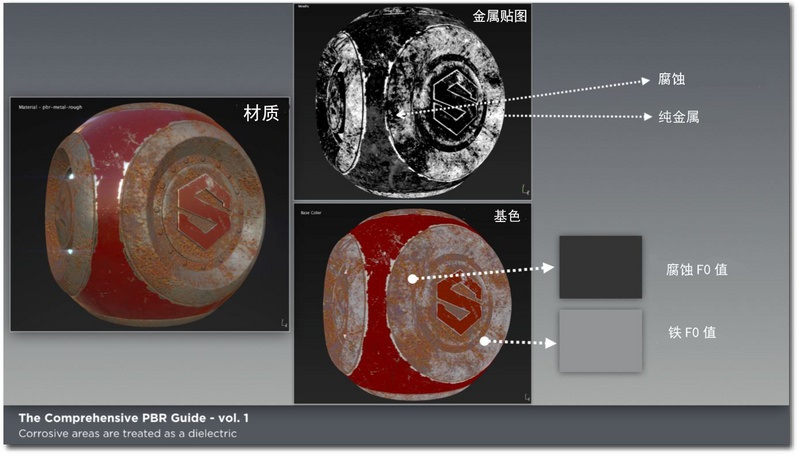
\includegraphics[width=\textwidth]{images/chap1_13.jpg}
	\caption{腐蚀区域被视作绝缘}
    \label{fig:chap1_13}
\end{figure}

同样,被涂漆的金属也会被当做绝缘物质看待。更准确的来说,被腐蚀的金属也是由于外层被涂上了一层绝缘物质的涂层(铁锈之类)。因此被天气影响的金属物质往往是导体和绝缘体的混合。

\section{非金属}

非金属是电的差导体或者绝缘体,光线在物体内部会同时存在散射和吸收现象(常常在散射后再次弹出物体表面)因此非金属反射的光的总量大大小于金属物质,因此非金属物质会有一张Albedo贴图来表示其本身的颜色(Albedo:反照率,表示物体反射和漫反射加起来对光线的反射程度),通常的绝缘体的零度角反射值F0只有2\%-5\%。这个值在PBR制作过程中的线性范围是0.017-0.067(40-75 sRGB值),如图\ref{fig:chap1_14}所示。除了宝石之外的大部分绝缘体不会超过4\%。

\begin{figure}[ht]
    \centering
	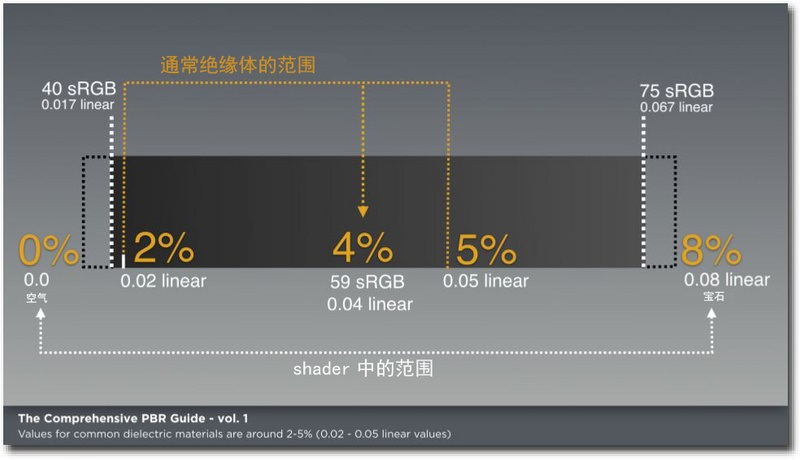
\includegraphics[width=\textwidth]{images/chap1_14.jpg}
	\caption{常见绝缘材质的值在2-5\%左右}
    \label{fig:chap1_14}
\end{figure}

和金属一样,我们需要去测量各种物质的反射值,然而不透明物体的折射率是很难测量的。好在各个非金属物质之间的数值差距是不大的,因此我们能用很少的几条准则去确定反射值。

\section{线性空间渲染(线性工作流)}

线性空间渲染是一个非常大的话题,我们不会深入讲解。重要的点在于所有的计算都需要在线性空间发生。

线性空间渲染保证了对于光照的计算的正确性,因为它保证了光线在计算机中的行为与在自然中的行为一致。
线性空间也就意味着gamma = 1.0。当然,为了人眼观看的正确,线性空间最后会被gamma矫正(人眼对光强度的感受不是线性的,超过一定亮度范围之后人眼的亮度感受会明显减弱)。gamma空间(sRGB)是图像最后在电脑屏幕上显示的空间,gamma空间中的RGB值都被调整过。
当计算颜色值或对颜色进行操作时,所有的操作也必须在线性空间进行。一个简单的标准就是,如果一张图需要最后在渲染窗口输出,比如颜色贴图,漫反射颜色贴图,那么它就必须被设置为sRGB格式。在substance软件中如果一个贴图被标记为sRGB,它在计算中会被自动转换为线性空间(digamma)并在显示时再转回来。然而,如果你在贴图中存储的是物体表面属性比如粗糙度之类,那么这些图的值必须是线性空间的。

Substance处理了线性空间到sRGB的自动转换,在viewport输出的结果会被自动进行gamma矫正。对于艺术家来说,不用担心对于线性工作流的集成工作,所有线性空间的转换工作都在substance的插件中完成了。

当然,理解这个过程的原理是很重要的,当用substance导出bitmap而不是substance material 时,你需要自己手动处理线性空间和sRGB的转换。你需要知道基本的颜色/漫反射贴图是sRGB格式剩下的贴图必须是线性格式。

\section{关键因素}

现在我们可以总结一下PBR的核心思想和关键因素:

\begin{enumerate}
\item 能量守恒。反射的光线绝对不会比入射光线亮,这个过程由shader控制。
\item 菲涅尔。BRDF由shader控制,F0反射值对于大多数非金属的范围是2\%-5\%,对于金属则高达70\%-100\%。
\item 高光强度由BRDF控制,受粗糙/高光贴图和F0反射值影响。
\item 光照计算必须在线性空间完成,shader中输入的gamma过的图比如漫反射贴图需要被转成线性空间,在具体操作时需要根据不同引擎和渲染器的不同做不同的操作。而描述物体表面属性的贴图如粗糙度,高光图,金属贴图等等必须保证是线性空间。
\end{enumerate}

\section{References}

\begin{enumerate}
\item \href{https://disney-animation.s3.amazonaws.com/library/s2012_pbs_disney_brdf_notes_v2.pdf}{Physically-Based Shading at Disney Brent Burley, Walt Disney Animation Studios.}
\item \href{http://www.cs.cornell.edu/~srm/publications/EGSR07-btdf.pdf}{Microfacet Models for Refraction through Rough Surfaces}
\item \href{http://seblagarde.wordpress.com/2011/08/17/feeding-a-physical-based-lighting-mode/}{Feeding a Physically-Based Shading Model by Sebastien Lagarde}
\item \href{http://hmi.ewi.utwente.nl/verslagen/capita-selecta/CS-Jimenez-Kwast-Daniel.pdf}{An Introduction to BRDF Models by Daniël Jimenez Kwast}
\end{enumerate}